\section{Hardware components}

Significant features and specifications of hardware used in this project will be noted in this section.

\subsection{Microcontroller}
The microcontroller chosen for this project is STM32F103C8T6. 
It's core is an ARM Cortex-M3 32-bit processor with a RISC instruction set. 
While the maximum oprating frequency of this chip is 72MHz it is also paired with 128KB of flash memory and up to 20KB of SRAM.\cite{STMDS}. 
This board is made by ST-Electronics\footnote{https://www.st.com/} and among the enthusiasts recognized under the name ``Blue pill''.

\begin{table}[htbp]
    \caption{Microcontroller dimensions}
    \begin{center}
        \begin{tabular}{|c|c|}
            \hline
            \textbf{Height} & \textbf{Width}\\
            \hline
            53mm & 23mm\\
            \hline
        \end{tabular}
        \label{tab1}
    \end{center}
\end{table}

M3 processors made by ARM\footnote{https://www.arm.com/} provide a cheap architecture which has low power comsumption levels which makes it a good choice for this type of projects.

\begin{figure}[htbp]
    \centerline{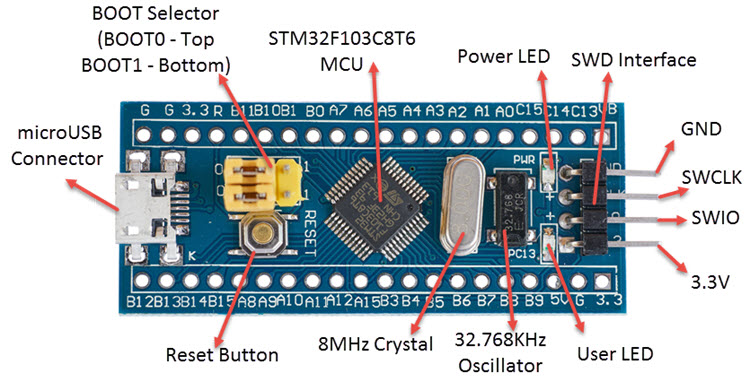
\includegraphics[width=8cm]{Images/STM32F103C8T6.jpg}}
    \caption{STM32F103C8T6}
    \label{fig1}
\end{figure}

The board itself has 48 pins with 37 of them being General-purpose I/O (PA0-PA15, PB0-PB15, PC13-PC15) and 15 of them supporting pulse width modulation (PA0-PA3, PA6-PA10, PB0-PB1, PB6-PB9). All digital pins have interrupt capability. The pins are separated into 3 ports, A, B and C. 

\subsection{Rotary encoder}

Rotary encoder is a device used for sensing rotation as well as the direction of the rotation. Even though there are many types of encoders that subject will not be covered in this paper. The rotary encoder used in this project is an absolute incremental encoder KY-040. The way absolute incremental encoders work is by having the controller sense two output signals (Clock and Deadtime pins). When the handle of the encoder is both of the signals are set to high voltage. The order in which the signals are triggered determines direction of the rotation. To sum this up, once the controller recieves interrupt on the first pin,direction of rotation can be determined by checking the state of the of the second pin.


\begin{figure}[htbp]
    \centerline{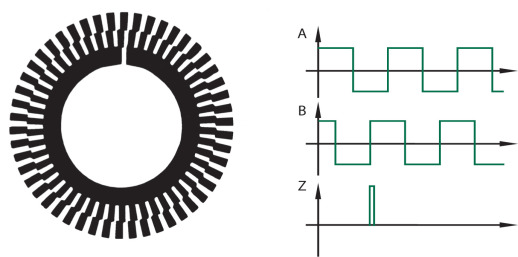
\includegraphics[width=8cm]{Images/Encoder.jpg}}
    \caption{Absolute incremental encoder}
    \label{fig2}
\end{figure}

Tha role of an encoder in this project is to tweak the speed of rovers wheels by turning it clockwise or counterclockwise.

\subsection{DC Motor}

DC motors are consisted of to key components: an armature (rotating part) and a stator (stationary part). By turning the electric into magnetic energy, this type of motor achieves rotation by turning its magneticly polarized shaft. The direction in which the shaft turns is determined by the direction of current flowing trough the motor. 

\begin{figure}[htbp]
    \centerline{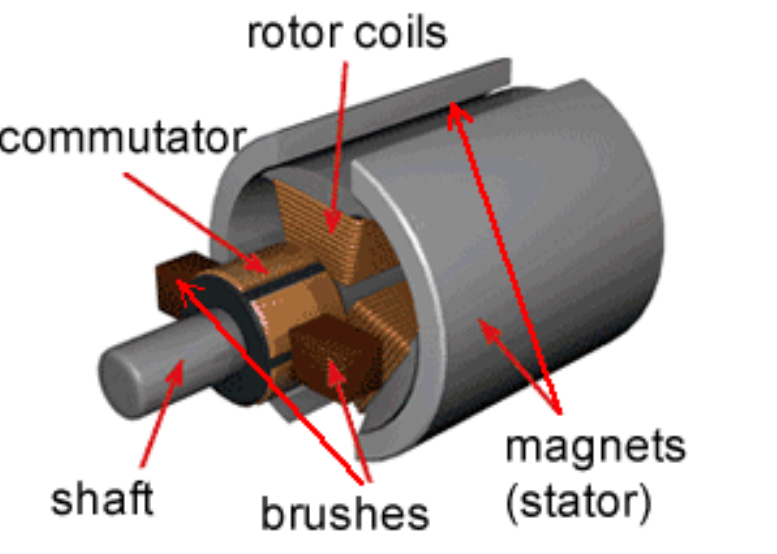
\includegraphics[width=8cm]{Images/DC.png}}
    \caption{DC Motor internals}
    \label{fig3}
\end{figure}

This project requires four DC motors, one for each wheel.

\subsection{Motor driver}

Changing the current flow in a DC motor to achieve rotation using a microcontroller is not a trivial task. This problem lead to development of an electric circuit which changes the polairity of applied voltage called the H-bridge. H-bridges consist of four switches which act as a device that can change the flow of current going thorough a motor.

\begin{figure}[htbp]
    \centerline{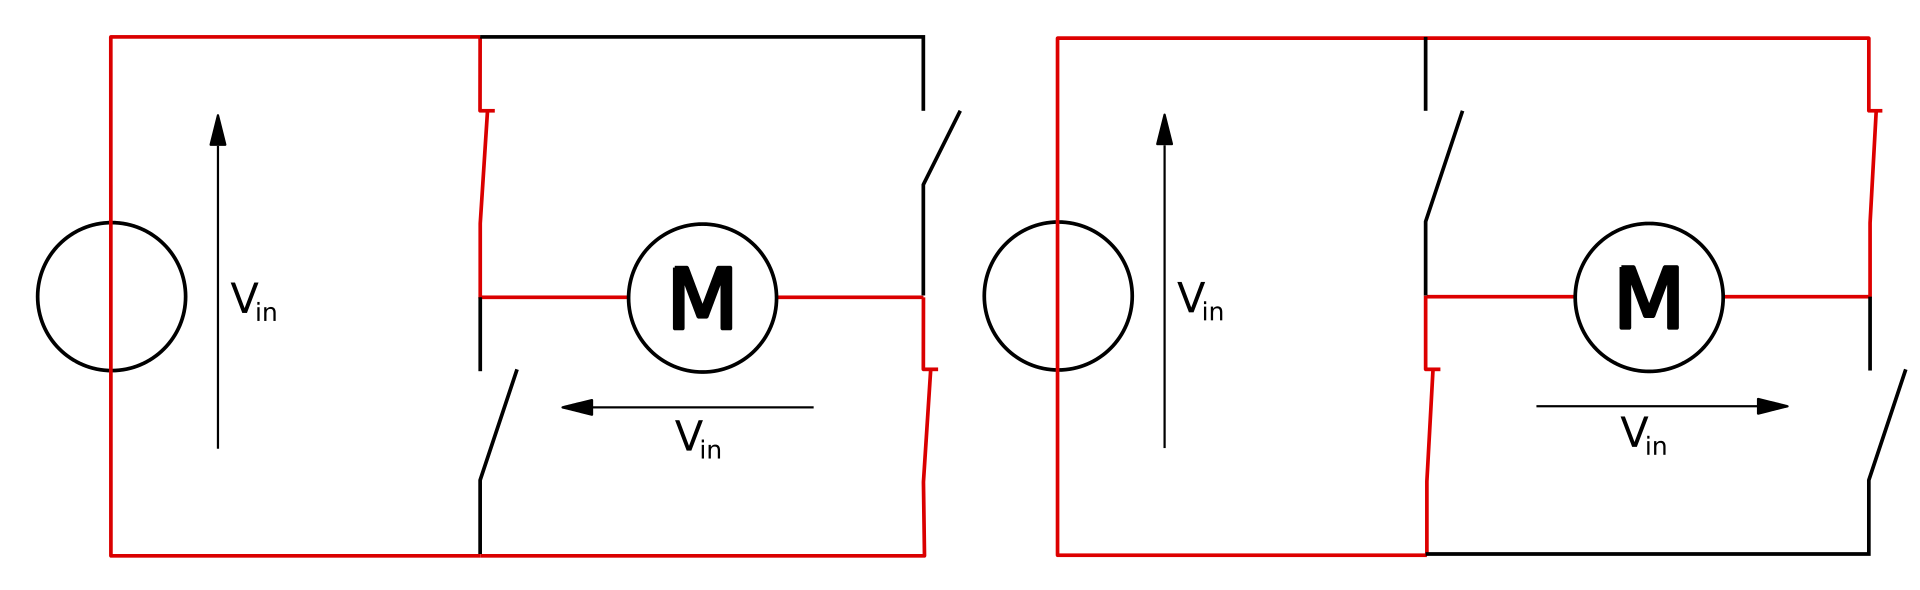
\includegraphics[width=9cm]{Images/H-Bridge.png}}
    \caption{H-bridge states}
    \label{fig4}
\end{figure}

A more complex component which resolves this problem is a motor driver. These components, such as L298N which was used in this project, have the ability to control when and in which direction the motor rotates. This type of motor driver is popular among hobbyists mainly due to its low price. L298N is a dual-channel driver meaning that it can run two motors simultaneously . The driver operates under 5V with the maximum power consumption of 20W\footnote{when the temperature T = 75 °C}. There are three main pins per motor with them being two input pins and an enbale pin. The purpose of enable pin is to connect a PWM\footnote{PWM - Pulse Width Modulation} to it in order to control the speed of a motor. Remaining two pins are used to determine the direction of rotation.\cite{L298N}

\begin{table}[htbp]
    \caption{Input pin combinations}
    \begin{center}
        \begin{tabular}{|c|c|c|}
            \hline
            \textbf{Input 1} & \textbf{Input 2} & \textbf{Direction}\\
            \hline
            HIGH & HIGH & None\\
            \hline
            HIGH & LOW & Direction 1\\
            \hline
            LOW & HIGH & Directino 2\\
            \hline
            LOW & LOW & None\\
            \hline
        \end{tabular}
        \label{tab1}
    \end{center}
\end{table}

Since this project requires four DC motors there will be two L298Ns runnig two motors each.

\subsection{Bluetooth module}

In order to control the robot there needs to be a way of communication. Since there is already an android app designed to control a robot of different purpose\footnote{https://www.gihtub.com/Adi-Sose/Fall-E} there is no need to look further for a solution. The solution for communication between devices is bluetooth. Most popular bluetooth module for these kind of projects is HC-05 and its newer version HC-06. HC-05 was the module used in this project due to its ease of use compared to HC-06 which is known to have some bugs. This module uses PSK\footnote{PSK- Phase Shift Keying} to communicate with other devices while UART\footnote{UART - Universal Asynchronous Receiver/Transmitter} protocol is implemented for the component to communicate with the rest of the circuit \cite{HC-05}. UART protocol utilizes one data channel which makes it slower compared to its counterparts I$^2$C\footnote{Inter-Integrated Circuit} and SPI\footnote{Serial Peripheral Interface} which is compensated by its lower resource usage. The HC-05 has two pins that support UART, recieve and transmit pin which are used for the circuit to send and recieve data outside of it through serial communication. 

\begin{figure}[htbp]
    \centerline{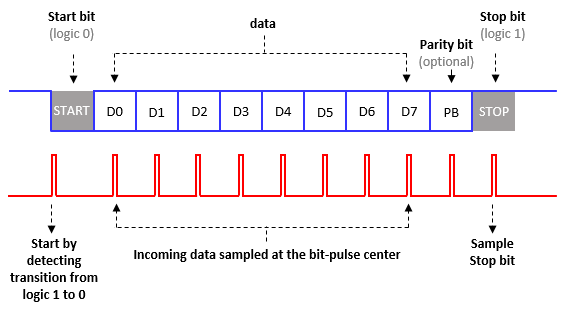
\includegraphics[width=9cm]{Images/UART.png}}
    \caption{UART Data Package}
    \label{fig5}
\end{figure}

The speed of this communication is 9600 bits per second.

\subsection{Ultrasonic Sensor}

For the rover to be able to detect obstacles some kind of distance sensor is needed. Widely available ultrasonic sensor family is the HC-SR type. The way in which the HC-SR04, component used in the project, works is by sending a 10µs signal to its trigger pin. Then an ultrasonic wave is sent from the device and once it is returned the distance can be measured by the time it took for the signal to return which is equal to the time that the echo pin will be set to its high state.\cite{HC-SR03} Since the speed of sound is 340$\frac{m}{s}$ a smiple equation can be created for calculating the distance.

\begin{gather}
    v = 340\frac{m}{s} = 0.034 \frac{cm}{\text{µ}s}\\
    t = \frac{s}{v}\\
    s = t * \frac{0.034}{2}
\end{gather}

Since the rover doesn't have a strict direction of movement there are two sensors of this type mounted on the front and the back of the robot.